\documentclass[conference]{IEEEtran}
%future work: local patch operator
%complexity

\usepackage{subfig}
\usepackage{wrapfig}
\usepackage{amsmath}
\usepackage{url}
\usepackage{pifont}
%\usepackage{times}
\usepackage{rotating}
%\usepackage{balance} 
\usepackage{color, colortbl}
\usepackage{graphicx}
\usepackage{algorithmicx}
\usepackage[running]{lineno}
\usepackage{program}
\usepackage{cite}
\usepackage{alltt}
\usepackage{balance}
\newcommand{\eq}[1]{Equation~\ref{eq:#1}}
\newcommand{\bi}{\begin{itemize}}
	\newcommand{\ei}{\end{itemize}}
\newcommand{\be}{\begin{enumerate}}
	\newcommand{\ee}{\end{enumerate}}
\newcommand{\tion}[1]{\textsection\ref{sec:#1}}
\newcommand{\fig}[1]{Figure~\ref{fig:#1}}
\definecolor{lightgray}{gray}{0.975}
\usepackage{fancyvrb}
\usepackage{stfloats}
\usepackage{multirow}
\usepackage{listings}
\usepackage{amsmath}  
\DeclareMathOperator*{\argmin}{arg\,min} 
\DeclareMathOperator*{\argmax}{arg\,max} 
%\usepackage[usenames]{xcolor}




\usepackage{color}
\newcommand{\colorrule}[1]{\begingroup\color{#1}\hrule\endgroup}

\definecolor{darkgreen}{rgb}{0,0.3,0}

\usepackage[table]{xcolor}
\definecolor{Gray}{rgb}{0.88,1,1}
\definecolor{Gray}{gray}{0.85}
\definecolor{Blue}{RGB}{0,29,193}
\newcommand{\G}{\cellcolor{green}}
\newcommand{\Y}{\cellcolor{yellow}}


\definecolor{MyDarkBlue}{rgb}{0,0.08,0.45} 
\newenvironment{changed}{\par\color{MyDarkBlue}}{\par}

\newcommand{\ADD}[1]{\textcolor{MyDarkBlue}{{\bf #1}}}
\newcommand{\addit}[1]{\begin{changed}\input{#1}\end{changed}}

\usepackage{color}
\usepackage{listings}
\usepackage{setspace}

\definecolor{Gray}{gray}{0.9}
\newcommand{\kw}[1]{\textit{#1}}
\newcommand{\quart}[4]{\begin{picture}(75,6)
	{\color{black}\put(#3,3){\circle*{2.5}}\put(#1,3){\line(1,0){#2}}}\end{picture}}
% New Commands

\definecolor{Code}{rgb}{0,0,0}
\definecolor{Decorators}{rgb}{0.5,0.5,0.5}
\definecolor{Numbers}{rgb}{0.5,0,0}
\definecolor{MatchingBrackets}{rgb}{0.25,0.5,0.5}
\definecolor{Keywords}{rgb}{0,0,1}
\definecolor{self}{rgb}{0,0,0}
\definecolor{Strings}{rgb}{0,0.63,0}
\definecolor{Comments}{rgb}{0,0.63,1}
\definecolor{Comments}{rgb}{0.5,0.5,0.5}
\definecolor{Backquotes}{rgb}{0,0,0}
\definecolor{Classname}{rgb}{0,0,0}
\definecolor{FunctionName}{rgb}{0,0,0}
\definecolor{Operators}{rgb}{0,0,0}
\definecolor{Background}{rgb}{1,1,1}
\title{Actionable = Cluster + Constrast?}

% You can go ahead and credit any number of authors here,
% e.g. one 'row of three' or two rows (consisting of one row of three
% and a second row of one, two or three).
%
% The command \alignauthor (no curly braces needed) should
% precede each author name, affiliation/snail-mail address and
% e-mail address. Additionally, tag each Slope of
% affiliation/address with \affaddr, and tag the
% e-mail address with \email.
%
% 1st. author
\author{Rahul Krishna, Tim Menzies\\
	Computer Science, North Carolina State University, USA\\
	\{i.m.ralk, tim.menzies\}\@gmail.com
	
	% use '\and' if you need 'another row' of author names
	% 4th. author
}


\pagestyle{plain}
\begin{document}
	\maketitle
	\begin{abstract}
		There are many
		algorithms for data {\em classification} such as  C4.5, Naive Bayes, SVM, etc.
		Are these enough for software data analytics? Or should we be supporting
		another kind of reasoning? For example, this paper does not answer 
		``what is'' (i.e. the standard classification problem), but instead  offers advice on ``what to change''.
		Two approaches for learning minimal, yet effective,  changes,  software
		artifacts are explored. Lessons learned are reported.
	\end{abstract}
	\begin{IEEEkeywords}
		Prediction, case-based reasoning, data mining, software engineering.
	\end{IEEEkeywords}
	
	\section{Introduction} 
	How should we handle ``unpopulular'' results
	for data analytics? For example, if a business manager is presented
	with a data mining result that troubles them (e.g. an estimate of
	development time that is distressingly long), what advice
	can we offer them on management actions to {\em change} hat estimate?
	
	This is an important question, and one with much currency in industry.
	In the summer of 2011 and 2012, one of us (Menzies) spent two months
	working on-site at Microsoft Redmond,
	observing data mining analysts.  He
	noted how Microsoft's data scientists
	discussed their data with  business users. 
	One surprising from that study was just how
	little time was spent  
	inspecting  of the output of data miners as compared to another process, which we call {\em peeking}.
	In {\em peeking}, analysts and users spend much time
	inspecting and discuss small samples of either raw or exemplary or synthesized project data.  Further, very little of those discussions were  focused on classification
	(the additional of a labels to some unlabelled data). Rather, much time
	was spent in those meetings discussion {\em what to do next}; i.e. trying
	to determine what could be altered to better improve some business outcome.
	
	That   Microsoft  study found two common ``peeking'' methods.
	In {\em data engagement meetings},
	users debated the implications of data
	displayed on a screen. In this way, users
	engaged with the data and with each other by
	monitoring each others' queries and check each others'
	conclusions.
	
	Another data analysis pattern observed
	at Microsoft was  {\em cluster + contrast} in which
	data is  reduced to a few
	clusters. Users are then just shown the delta between those
	clusters. While contrasting, if feature values are
	the same in both clusters, then these were pruned from
	the reports to the user. In this way, very large
	data sets can be shown on one PowerPoint
	slide. Note that {\em cluster+contrast} was a tool that can be usefully employed within
	{\em data engagement meetings}.
	
	
	Cluster+contrast and engagement
	meetings are common practices at Microsoft. Yet  these methods had never been rigorously studied or certified.
	For both those reasons,
	we reflected over those tools to discover and analyze their
	underlying process. The result was HOW: a tool
	that combines (a)~feature selection; (b)~centroid generation from   clusters;
	(c)~contrast methods between centroids.
	While method (a) is widely used (e.g.~\cite{Menzies2010}),
	to the best of our knowledge, this combination of (abc) has not been thoroughly explored before.
	Hence, this paper explores ``peeking''.
	
	\section{ Evaluating Changes to a Software Project}
	
Before beginning, we offer three comments on evaluating changes to a project.
Firstly, a planning system needs to be {\em effective}; i.e. if its recommendations
are applied then some statistically significant change should be observed.
To predict the number of defects in a data set before and after applying our changes,
we build a    prediction system (built by data mining; specifically: CART). Note that this
predictor was built from some hold-out data (i.e. from  different data than that used
to build the predictor).

Secondly, an important evaluation criteria for any conclusion made to a business user is that the users can understand the proposed change. In practice, this means at least
generating {\em succinct} changes. As seen below, not all cluster+contrast methods generate succinct changes.

Thirdly, as a final evaluation criteria, we will demand that the generated recommendations are {\em stable}; i.e. do not widely vary due to minor changes in the data. Hence, in the following, we will add a little randomness to our analysis then report results across 20{\bf XXX} repeated runs. In a result that supports our kind of analysis, we will show that the actions proposed by this analysis are very stable.

	
	\section{How to Cluster}
	Recent results suggest  we are free to select from a wide range of 
	clustering methods.  Ganesan~\cite{div14} explored 
	different clustering methods for SE data using   effort and defect data from
	the PROMISE repository\footnote{http://openscience.us/repo};
	That studied explored
	K-Means, mini-batch-K-Means, DBscan, EM, Ward, and the WHERE algorithm discussed
	below.
	Clusters were assessed via the performance of prediction 
	learned from the clusters by Random Forests (for defect prediction)
	and M5prime or linear regression (for effect estimation).  Ganesan found
	that the details of the clustering method were less important than ensuring that  a large number of clusters were generated.
	
	Accordingly, we select a clustering method that generates $\sqrt{N}$ clusters
	from $N$ examples, that runs fasts, which has shown promise in prior work~\cite{Menzies2013}, and which ignores spurious dimensions (the last item is important since, in our experience, much SE data is ``noisey''; i.e. contains signals not associated with the target variable). For the rest of this article,
	we use  the top-down
	bi-clustering method described in \fig{where} which recursively divides the
	data in two  using a dimension that captures the greatest variability in the data. 
	\begin{figure}[t]
		\small
		~\hrule~
		
		{\bf Step1: Top down clustering using WHERE}
		
		The data is recursively divided in clusters using WHERE as follows:
		\begin{itemize}
			
			\item Find   two   distance cases,  $X,Y$
			by picking any case $W$ at random, then setting $X$ to its most
			distant case, then setting $Y$ to the case most distant from
			$X$
			(this requires only $O(2N)$ comparisons
			of $N$ cases).
			\item Project each case $Z$
			onto a {\tt Slope} that  runs between $X,Y$ using the cosine
			rule. 
			\item Split the data at the median $X$ value of all cases and
			recurses on each half  (stopping when
			one half has less  than $\sqrt{N}$ of the original population).
		\end{itemize}
		~\hrule~
		
		{\bf Step2: Constructing Decision Trees}
		Call each leaf from WHERE a  ``class''. Use an entropy-based
		 decision tree (DT) learner to learn what attributes select for each ``class''. To limit tree size:
		 \bi
		 \item Only use the top $\alpha=33$\%  of the features, as determined by their information gain~\cite{Irani1993}. 
		 \item Only build the trees down to  max depth of $\beta=10$.
		 \item Only build subtrees if it contains at least $N^{\gamma=0.5}$ examples (where $N$ is the size of the training set).
\ei
{\em Score}  DT  leaf nodes  via the mean score of its majority cluster. 
		
		~\hrule~
		
		{\bf Step3: Generating contrast sets}
		\begin{itemize}
		\item Find the {\em current } cluster: take each test instance, run it down to a leaf in the DT tree.  
		\item Find the {\em desired} cluster: 
		\bi
		\item Starting at {\em current}, ascend the tree $lvl\in \{0,1,2...\}$ levels;
		\item Identify {\em sibling} clusters; i.e. leaf clusters that can be reached from level $lvl$ that are not {\em current }
		\item Using the {\em score} defined above, find the {\em better} siblings; i.e. those with a {\em score} less than $\epsilon=0.5$ times the mean score of {\em current}. If none found, then repeat for $lvl += 1$
		\item  Return the {\em closest} better sibling where distance is measured between the mean centroids of that sibling and {\em current}
		\ei
		\item Find the {\em delta}; i.e. the set difference between  conditions in the DT branch to {\em desired} and {\em current}. To find that delta:
		\bi
		\item
		For discrete attributes,  return the value from {\em desired}. 
		\item
		For  numerics, return the numeric difference. 
		\item
		For numerics  into ranges, return a random number selected from the low and high boundaries of the that range.
	\ei
	\ei
		~\hrule~
		\caption{Contrast tree generation: controlled by the parameters
		$\{\alpha, \beta, \gamma, \delta, \epsilon\}$ (set via engineering judgement).}
		\label{fig:contast_trees}
	\end{figure}
	
	\section{How to Contrast}
	Once we have  clusters, the next task is to offer business users lessons learned from comparing different clusters.
		Once methods for doing so are the {\em contrast trees} and the {\em instance-based}
		methods discussed below.
	
		\subsection{ Contrast Trees}

Contrast trees were first developed by Lekkalapudi and Menzies as a method
for explaining reasoning within multi-objective optimization~\cite{nva14}. This paper is the first
application of contrast trees to defect prediction.

	Contrast trees start by clustering data to find clusters $C_1,C_2,...$.
	Next, using those clusters as class labels, we execute a decision tree algorithm to find what attributes select for different clusters. After that, to learn recommendations for a business user, we determine (1) what {\em current} cluster are you in?; (2) what {\em desired} cluster do you want to move to?; (3) what is the delta between those clusters? To answer the last question, we report the delta in the branches of the decision tree that lead to {\em current} and {\em desired}.  For full details, see \fig{contast_trees}.
	
	%Contrast trees are decision trees that can be used to learn decision rules from a large data set. The use of decision trees for this purpose makes it easy to visualize the data and also makes interpretation of the recommended policies fairly straight forward. In addition to this, contrast tree generate ranges of decisions that allow for better feasibility.
 
 
	

As with any tree structure, the size and depth of the contrast tree has a profound impact on it performance. Our initial motivation was that the trees could serve as a medium for experts to identify and explore solution spaces that were local to the problem. The size of the decision tree, if too large, jeopardizes the readability of the solutions by increasing the complexity. We have therefore made efforts to reduce the size of the tree using  a pruning method that prunes away irrelevant branches that do not contribute better solutions (see step2 of \fig{contast_trees}). The smaller trees are much easier to understand.



	\subsection{Instance-based Contrasts}
	Contrast tree represents the next generation of our efforts to use contrast set learners for planning and case based reasoning. All the other methods were {\em instance-based methods}. 
	Instance-based methods,   reason directly
	from the loaded training data without first summarizing that data into a model.
	The opposite to an instance-based method is one that builds
	a model from the data, then reasons across that model (e.g. as done by
	contrast trees, above). 
	
	Our previous experiment with instance-based planning
	results in  W2. This was an instance-based planner that reflected over the delta of raw attributes \cite{6600685} (without any initial clustering). However, it frequently suffered from an optimization failure. When its plans were applied, performance improved in only $\tfrac{1}{3}$rd of test cases. 

	We conjectured that W2 was failing since it could not generalize over sufficient
	data. Hence, our next experiment was IDEA~\cite{me12c} which first clustered the data with WHERE (see step1 of  \fig{contast_trees}). IDEA made the mistake of summarizing the learned clusters via their median centroid (we now know that to be a mistake since, on experimentation, we found
	IDEA's optimization failures to be as frequent as those of W2).
 
The instance-based learner used in this paper is called HOW.
During training, HOW  (a) clusters the training data with WHERE; (b) assigns a unique id to each cluster; then  (c) find the median centroid of each cluster.
Next,  working in a random order, HOW labels each cluster with id of the  nearest cluster (that has yet to be labelled). This results are {\em partners}  of nearby clusters.
After that, HOW draws a {\em slope} between the centroids of each partner
then add a direction to that {\em slope}
such that ``up hill'' now points to the centroid of the cluster with a score that is
comparatively better than its partner.

When using HOW on test data, each test instance finds its nearest slope then follows
the slope ``up hill'' to find the best centroid in its local region.
The delta between that test instance and the best centroid is then HOW's
recommendation on how to improve that test instance.

	

	\begin{figure}[t]
		{\footnotesize  \begin{tabular}{{llrrc}}
				\arrayrulecolor[gray]{.90}
				\rowcolor[gray]{.95} \textbf{Rank} & \textbf{Treatment} & \textbf{Median} & \textbf{IQR} & \\
				1 &     Ant (Tree) &    0.67  &  0.41 & \quart{0}{39}{37}{69} \\
				1 &     Ant (HOW) &    0.7  &  0.13 & \quart{33}{13}{40}{69} \\
				1 &   Jedit(HOW) &    0.72  &  0.25 & \quart{25}{24}{42}{69} \\
				1 &   Jedit (Tree) &    0.75  &  0.13 & \quart{37}{12}{43}{66} \\
				\hline \end{tabular}}
		
		\caption{Results comparing the performance scores on sample projects from the Jurezcko data sets.}
		\label{fig:res}

	\end{figure}
	
	
	\begin{figure*}[!t] 
		\begin{minipage}{0.5\linewidth}
			\subfloat[Contrast tree learning]{
				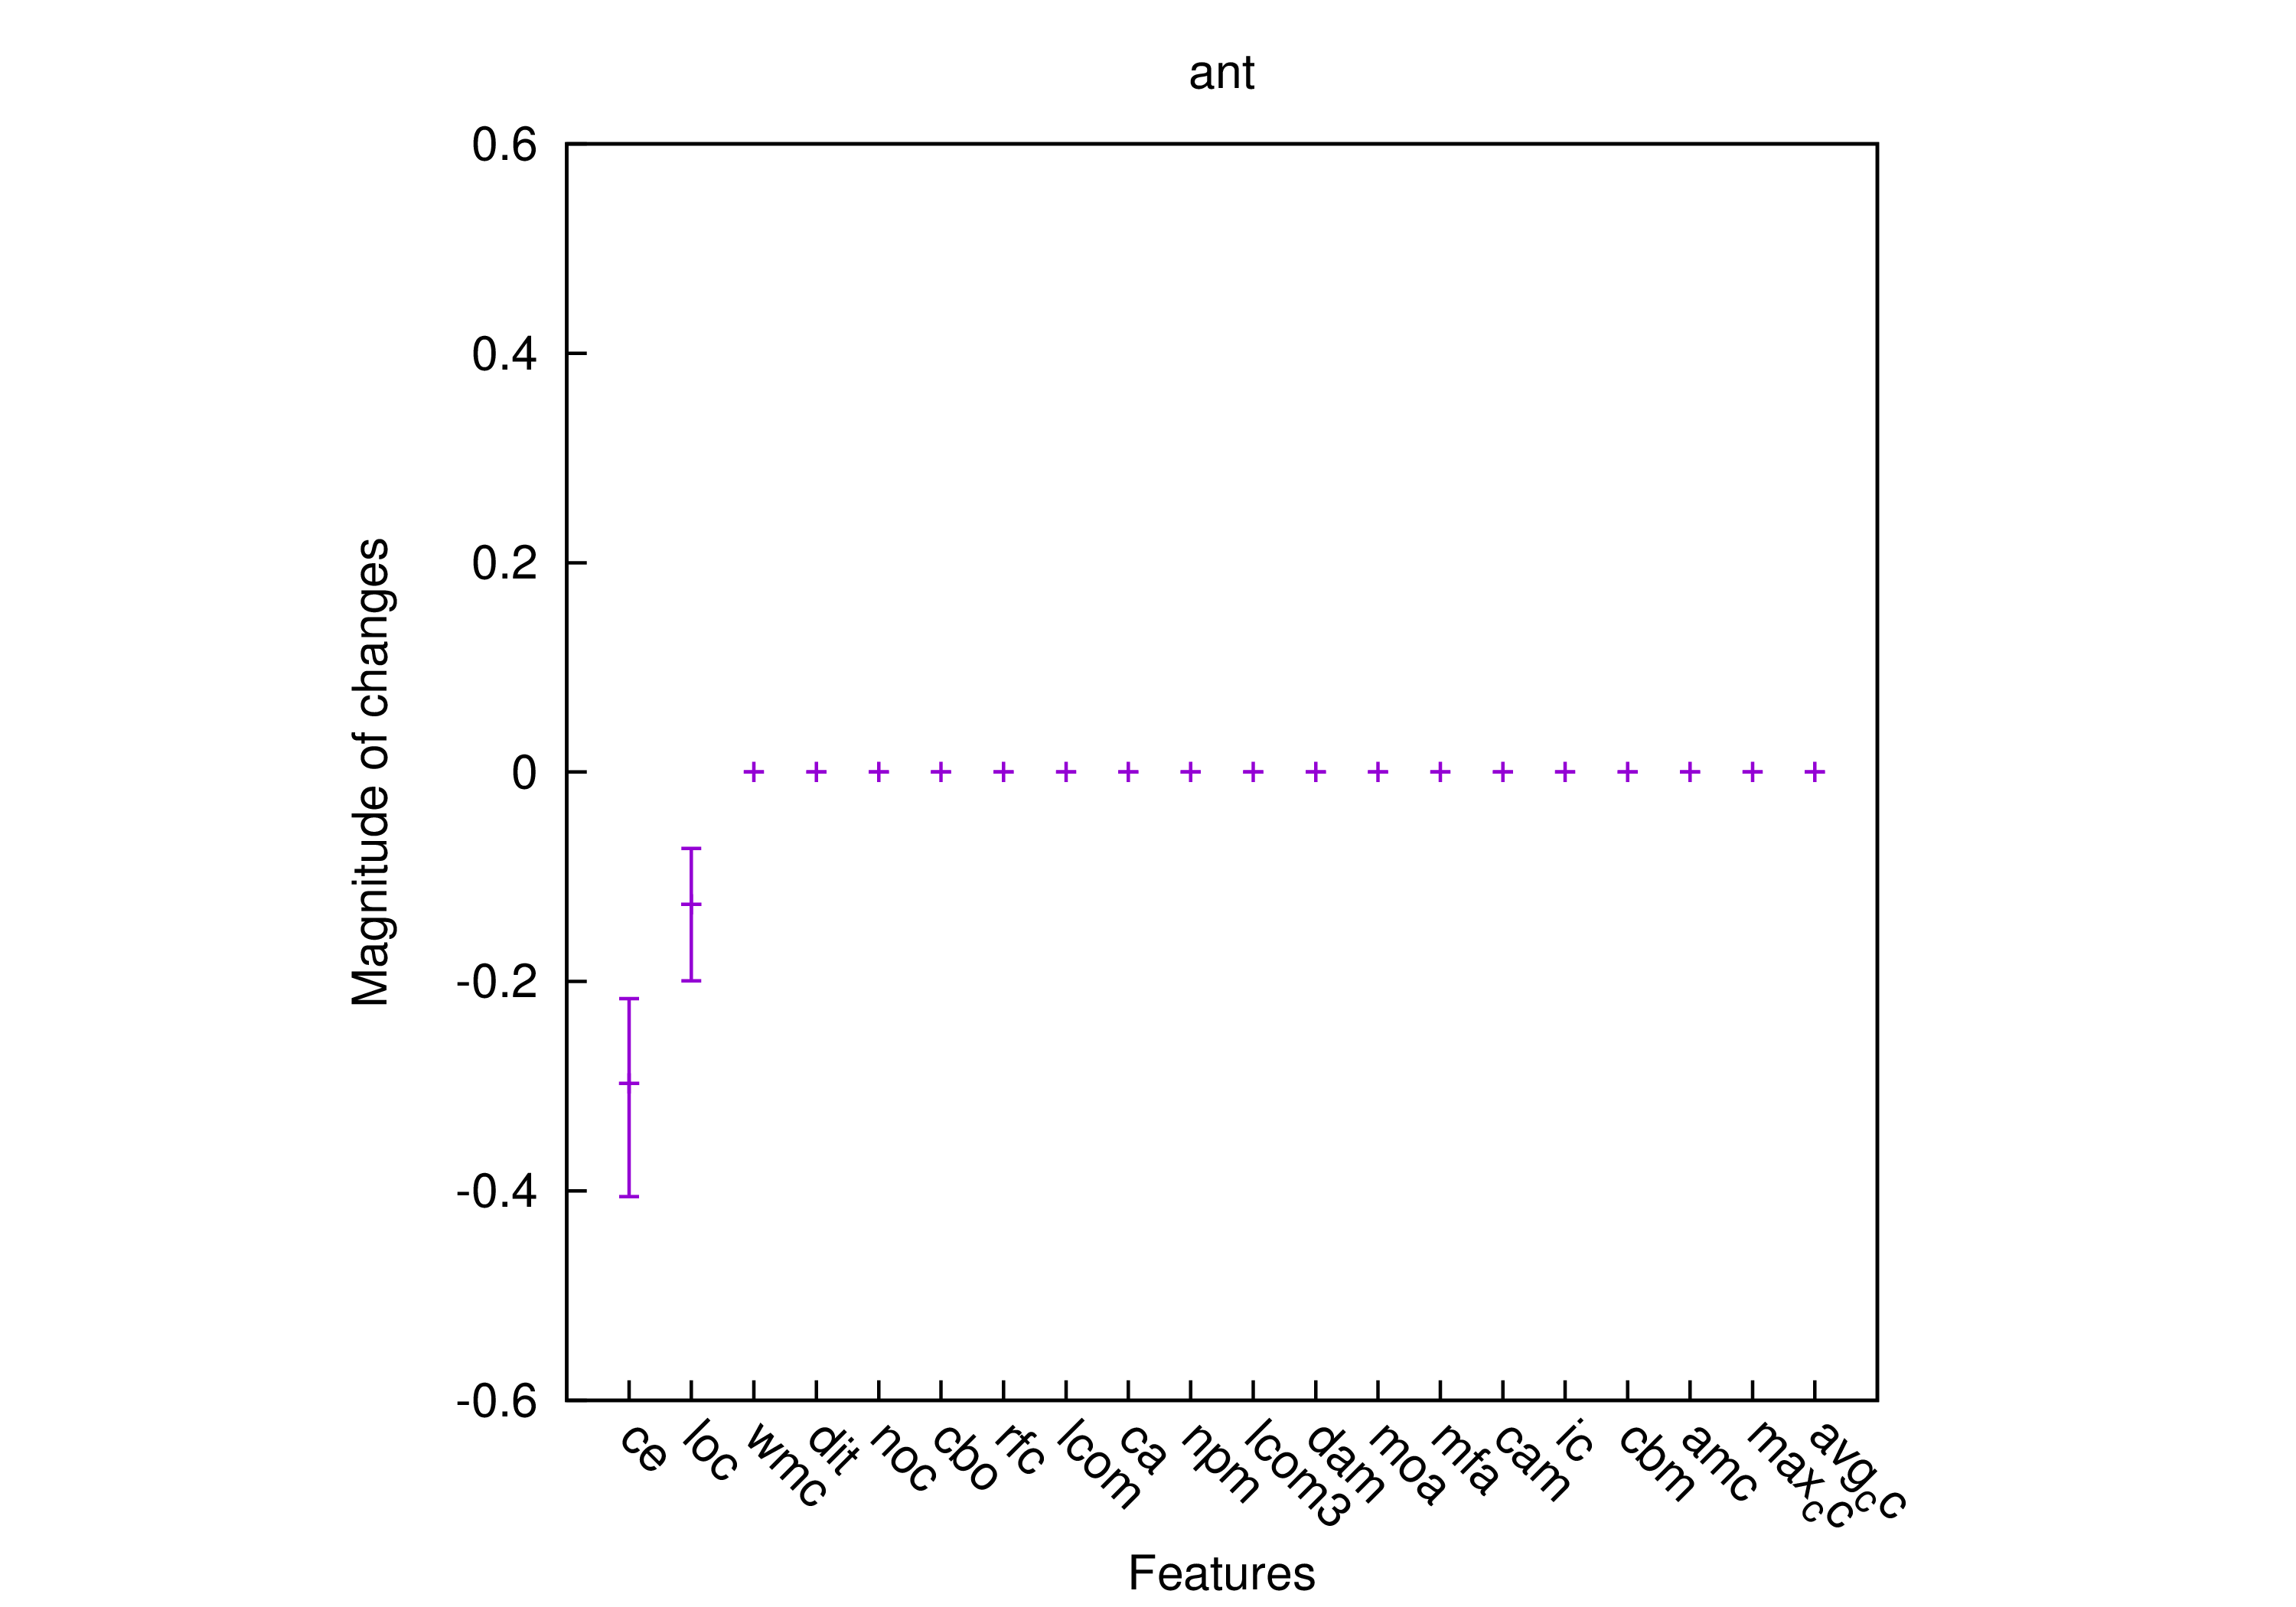
\includegraphics[width=\linewidth]{ant1.png}
				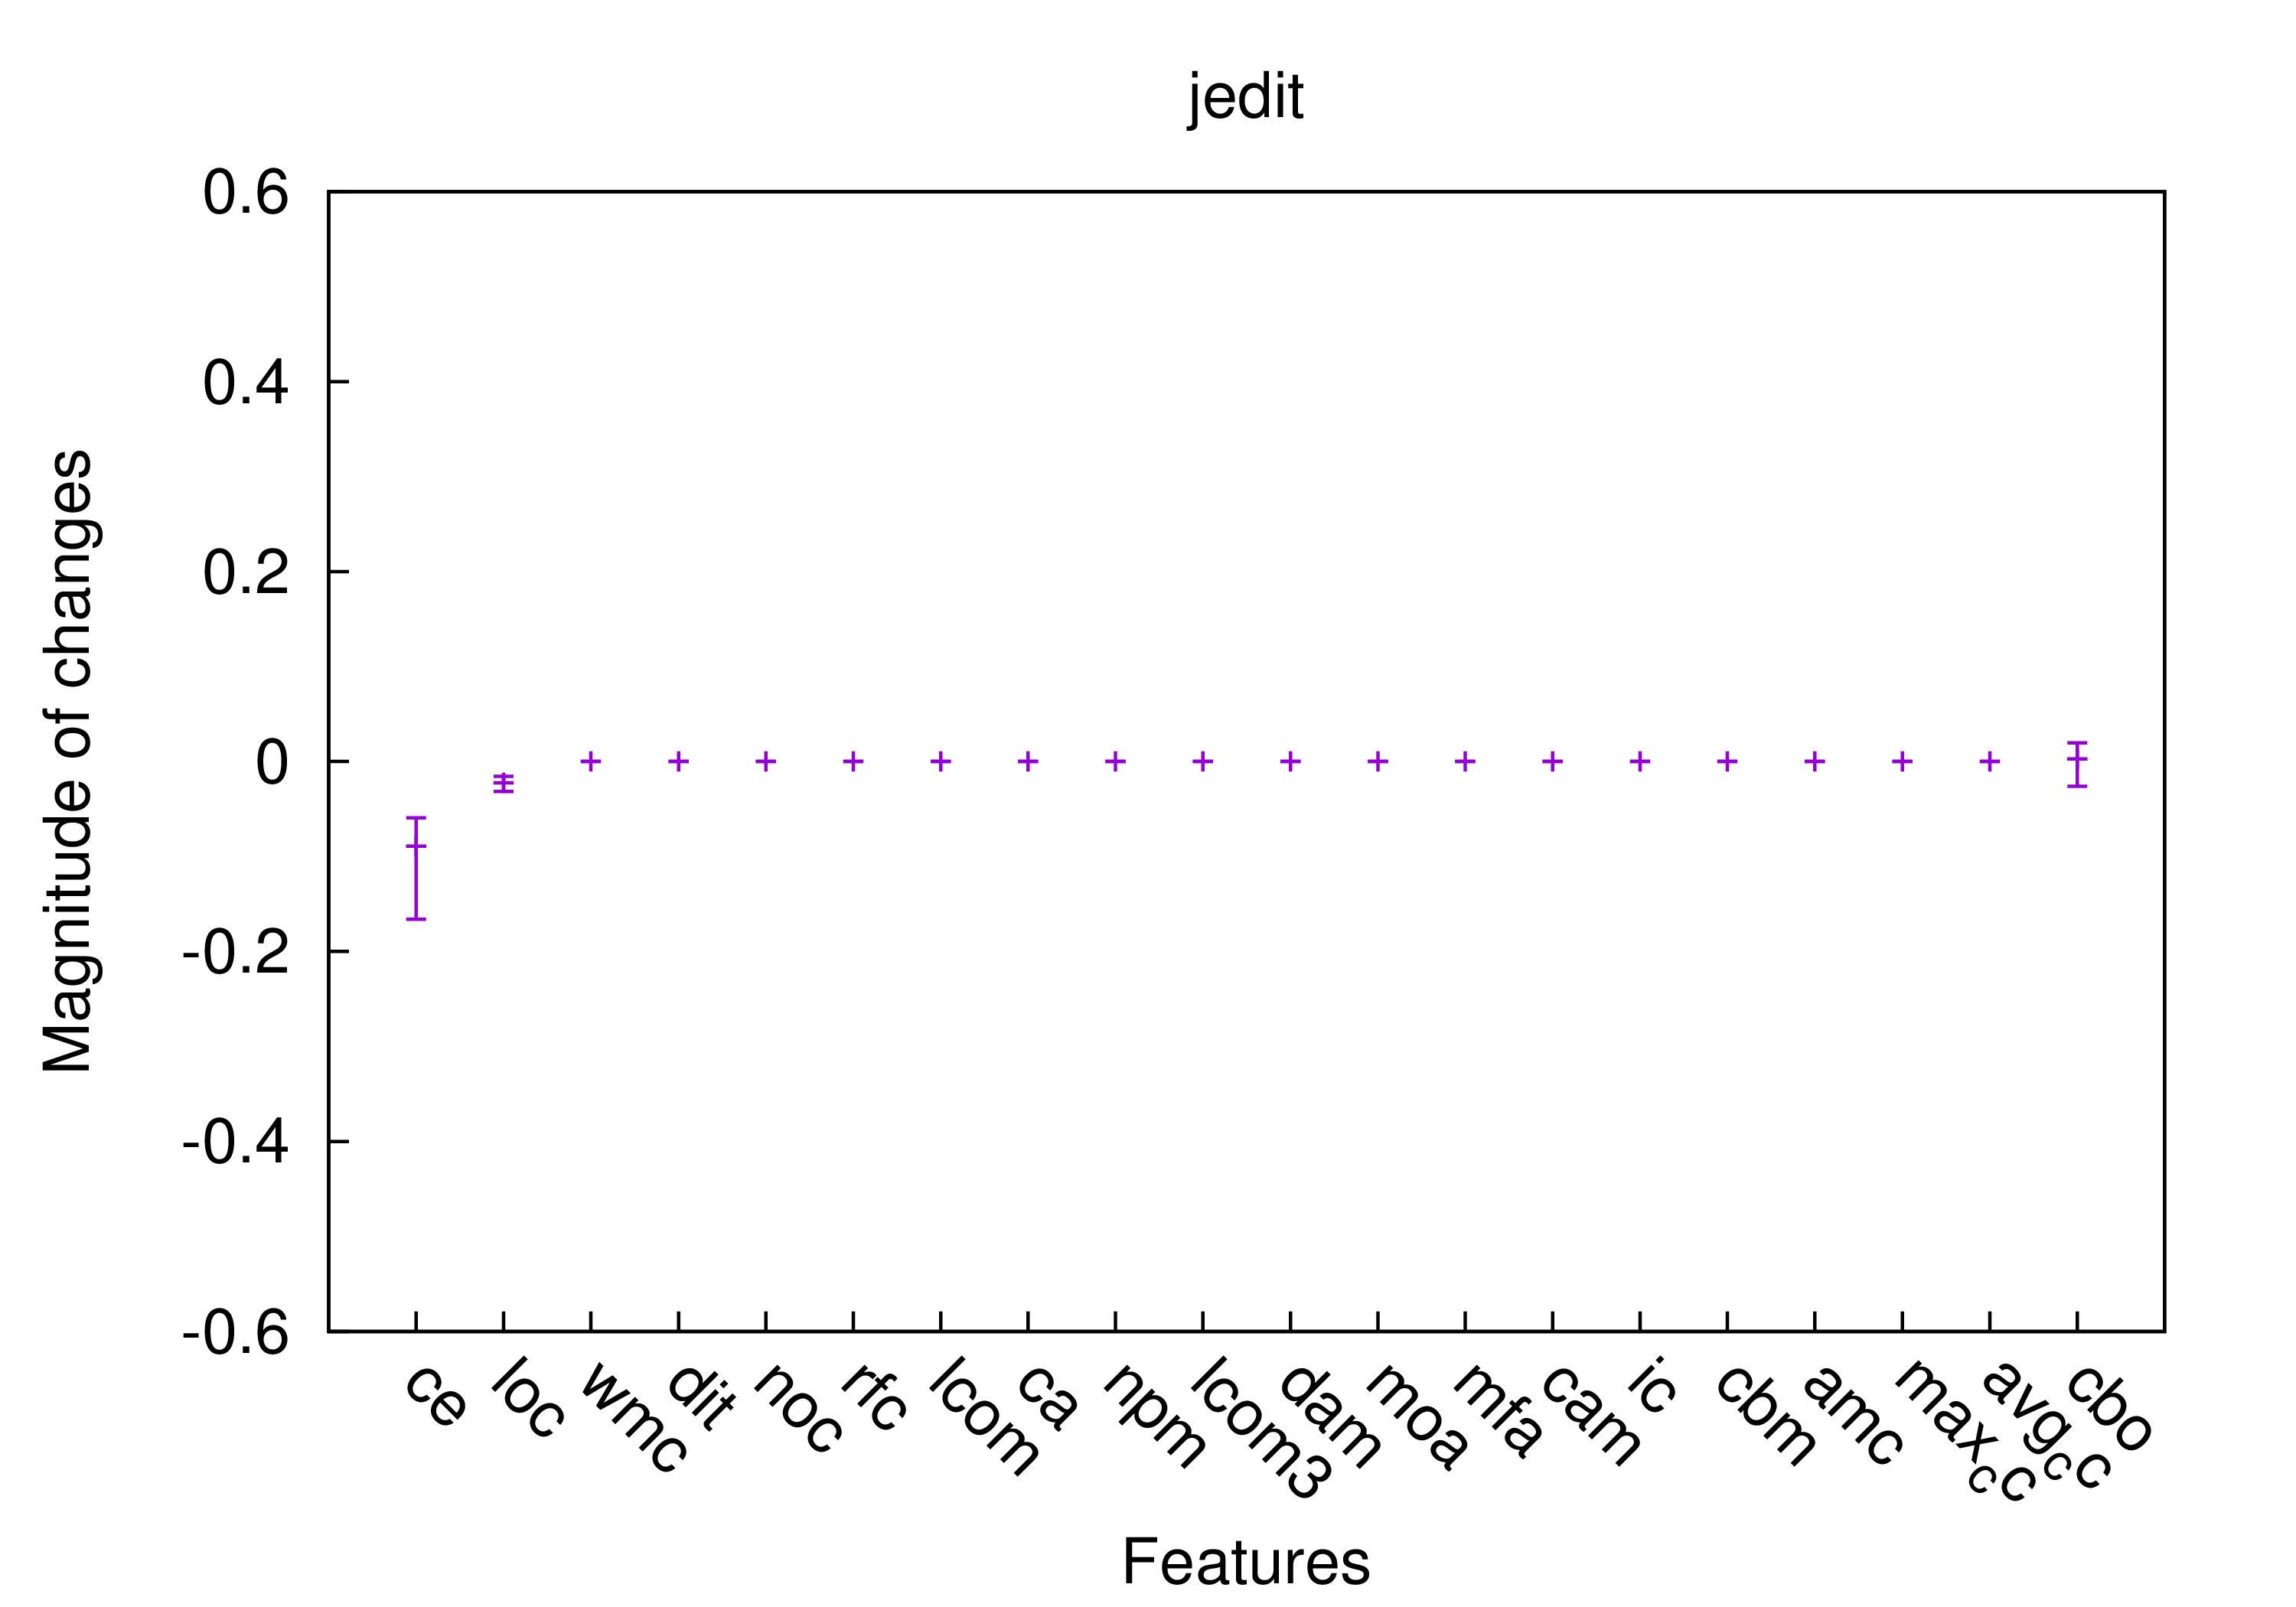
\includegraphics[width=\linewidth]{jedit1.png}}\\
			\subfloat[Instance-based contrast sets]{			
				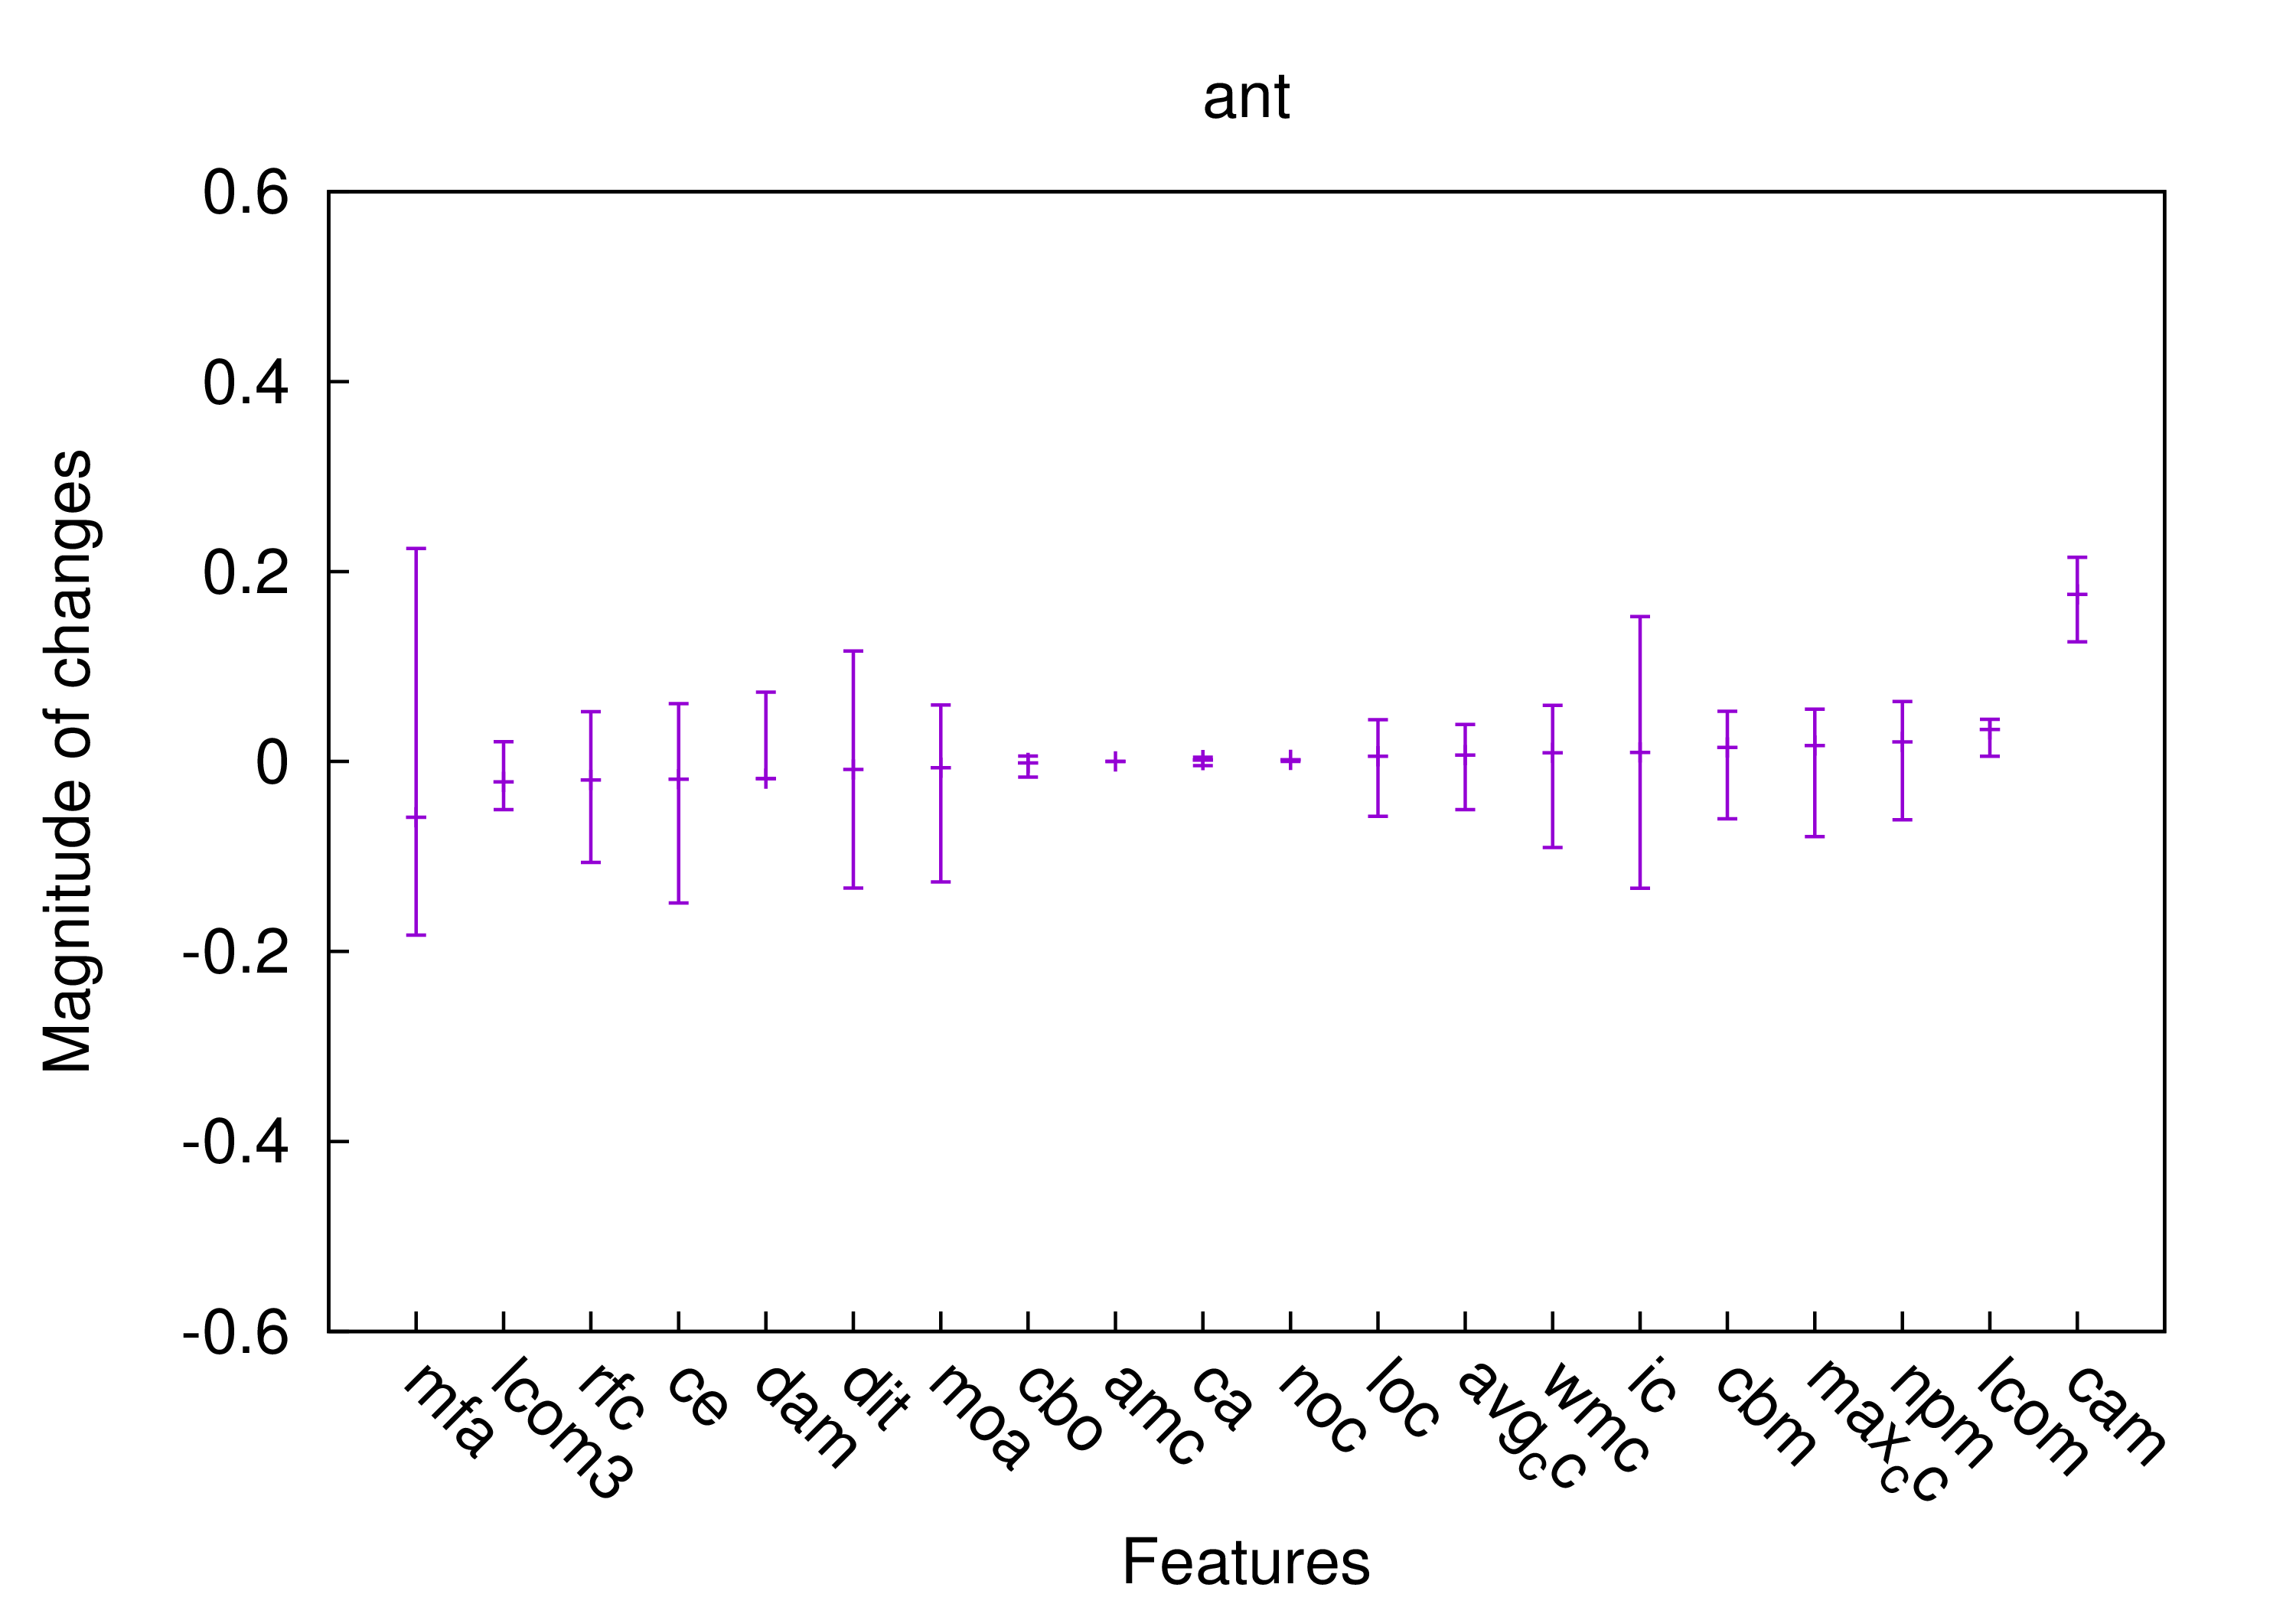
\includegraphics[width=\linewidth]{ant2.png}
				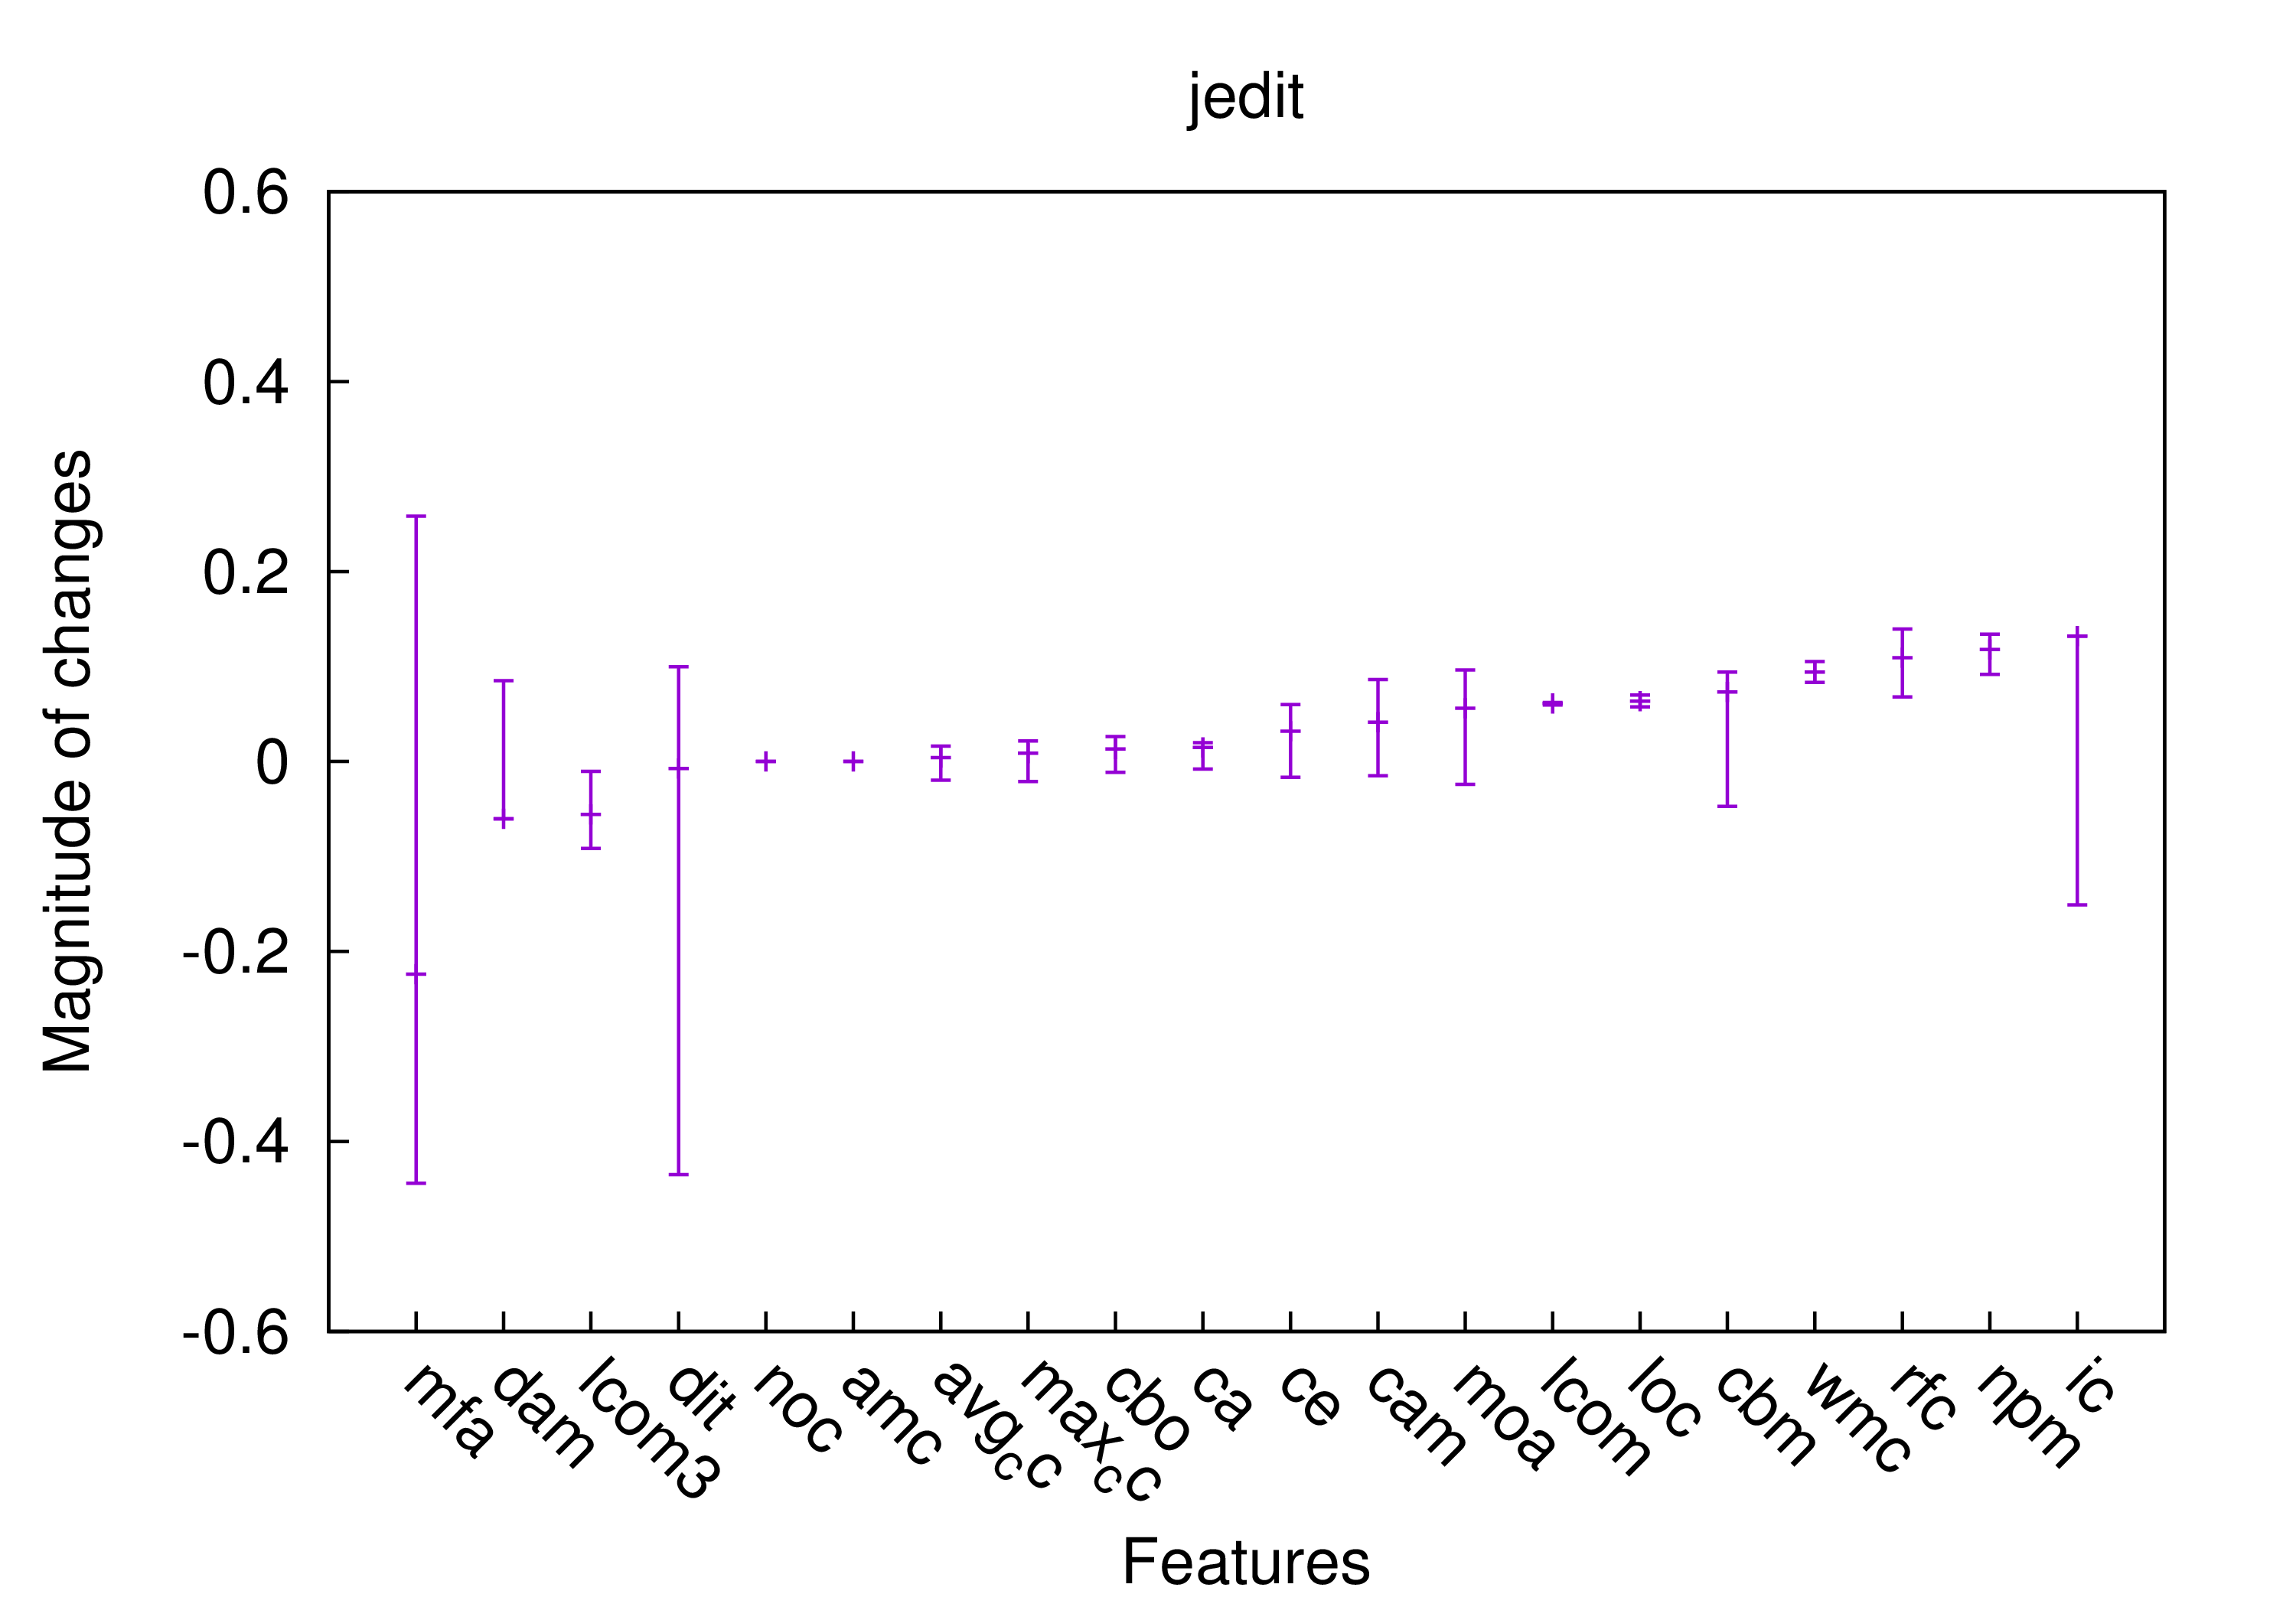
\includegraphics[width=\linewidth]{jedit2.png}}
		\end{minipage}
		\caption{Performance Comparison.
		X-axis lists various CK metrics such as loc (lines of code),
		ce (how many other classes are used by a specific class),
		cbo (class coupling, measured by number of methods accessing
		the services of another class). Top row shows results from contrast
		trees; bottom from instance-based methods. The attributes (on the x-axis)
		are sorted according the distribution of the changes recommended by 
		our two instance-based planners (most negative on left; most positive on right). The vertical bars in these charts indicated 25th, 50th, 75th precentil of the size of changes proposed by the different methods.}
		\label{fig:deltas}
	\end{figure*}
	
	
	\section{Experiments}
	\subsection{Data}
	For our initial experimentation, we studied two sample projects from the Jureczko object-oriented static code data sets~\cite{jureczko10}: Ant and  Jedit\footnote{Available from the object-oriented defects section of the PROMISE repository openscience.us/repo/defect/ck.}. The data is a collection of 20 OO measures and a the Boolean dependent attribute (whether a defect is reported to a post-release bug-tracking system). 
	
	\subsection{Analysis Methods}
	Recall from earlier in this paper, we proposed assessing instance-based planner
	via their {\em effectiveness}, {\em stability}, and  {\em succinctness}.
\bi
\item
	To assess {\em effectiveness}, all our results are  presented as ratios of the number of defects seen $\frac{\mathit{after}}{\mathit{before}}$ applying the recommended  (so numbers less than 1.0 indicate improvements). 
	\item
	To test for {\em stability}, we introduce some small randomness into our recommender systems, then re-run our experiments twenty times (the value of 20 was chosen as the minimum use sample size via the central limit theorem). Our randomness comes from WHERE's initial stochastic selection of instances (recall step1, discussed above) and from the random partner discovery procedure of HOW.
	\item
	To test for {\em succinctness}, we count the frequency and size of attribute changes recommended by contrast trees or HOW.
	\ei
To test if the distributions generated by the above are truly different, we
used the the Scott-Knott procedure recommended by Mittas \& Angelis in their 2013
IEEE TSE paper~\cite{mittas13}. The samples for the Scott-Knott are  obtained by repeating our experiments at least 20 times. With Scott-Knott, when testing for significant differences between samples, we used an see Efron \&
Tibshirani bootstrap procedure~\cite[p220-223]{efron93} augmented with an A12 effect size test (and distributions were only ranked  different if that difference was recognized by
both bootstrapping and the effect size test).

\subsection{Results}
	
\subsubsection{EFfectiveness}
The results of figure \ref{res} shows that for our test data, Contrast Trees and HOW are equally effective. Hence, to compare these methods, we have to look
beyond effectiveness towards stability and succinctness.

\subsubsection{Succinctness}

\fig{deltas} shows the distribution of changes prosed by contrast trees
and instance-based learning.  Note that contrast trees fare better in terms
of succinctness since the contrast trees propose changes to {\em far fewer attributes}
than instance-based methods.

\subsubsection{Stability}
\fig{deltas} also shows that the above succinctness result is stable across
our 20 repeated runs. Further, comparing the sum of  the size of all the changes proposed in the top and bottom row of \fig{deltas}, we can see that the recommendations of contrast trees are far less varied than those of instance-based contrast methods.
 
 \section{Summary and Future Work}
For the purposes of finding changes  we recommend
contrast trees over instance-based methods:
	
	\begin{itemize}
		\item Contrast trees allow the user to exert a fine grain control over the parameters that needs to be changed, while providing a way to visualize the recommended changes.
		\item The changes suggested by the contrast sets are inherently local in nature (specialized to each test instance), making the changes practical and potentially easy to implement.
	 
	\end{itemize}



 
\bibliographystyle{plain}
\bibliography{hownot}
\end{document}